\section{Introduction and Project Motivation}
\label{sec:intro}

Machine learning is written in Python and made fast in C++. OxCaml~\cite{oxcaml},
Jane Street's performance-oriented branch of OCaml, is built to test whether a
high-level, garbage-collected, type-safe language can run close to C++ when the
programmer can \emph{opt in} to performance. This project asks a narrow,
measurable version of that question: running one small language model's
inference on a single CPU core in five languages that compute the same thing
under one numerical contract, \emph{where does OCaml lose time to C++, and how much can be won
back in the source, the runtime and the compiler?}

The workload is Andrej Karpathy's \code{microgpt.py}~\cite{karpathy_microgpt},
a dependency-free GPT trained on 32,032 first names~\cite{karpathy_makemore}.
I ported its inference to C++, Rust, OCaml and OxCaml, built a benchmark that
checks the ports agree in every printed digit, and then closed the gap between
OxCaml and C++, each step chosen by what the previous one measured.

\subsection{Initial Approach: Novel CPU Inference in llama.cpp}
\label{sec:intro-llamacpp}

The first three weeks of August went into looking for a novel change to CPU
inference in \code{llama.cpp}~\cite{llamacpp}, the standard C/C++ engine for
running language models on CPUs.

\paragraph{KV-cache compression.} The first proposal was to compress cold
key--value cache entries on idle cores during decoding. Following my guide's
suggestion, I first implemented existing schemes: StreamingLLM-style
eviction~\cite{xiao2024streamingllm} and a reformulation of KIVI's per-channel
key quantisation~\cite{liu2024kivi}. Evicting one token per step made decoding
42\% \emph{slower}, and batched eviction was still 11\% slower despite 69\%
fewer resident tokens, because attention scans the cache's \emph{physical} span
and \code{llama.cpp} never compacts the holes that eviction leaves.

\paragraph{Algorithmic ideas.} Eight further ideas (activation sparsity,
speculative decoding, Barnes--Hut style summaries of KV pages, prefetching, and
others) were each ruled out by a cheap measurement of their assumption: for
example, only 0.7\% of feed-forward neurons can be skipped in blocks of 64,
although 32\% are individually inactive.

\paragraph{A focused workload.} In a heavily optimised engine a new idea is
either prior art or quickly settled by measurement. The project therefore
moved to a workload small enough to understand instruction by instruction,
where the variable is the \emph{language and its compiler}, measured with a
paired, pinned, interleaved protocol (Section~\ref{sec:method}).

\subsection{Core Goals}
\begin{itemize}
  \item Port microgpt inference to four languages with \emph{bit-identical}
        output, verified by a hash.
  \item Measure throughput fairly, each optimisation a separate build variant.
  \item Find at the instruction level why OCaml is slower than C++, and close
        the gap in the source, the runtime and the OxCaml compiler.
  \item Check that the compiler changes generalise, on a numerical library
        (nx-oxcaml) and a cryptography code base (oxcaml-crypto-study).
\end{itemize}

\subsection{Summary of Outcomes}
All gaps are throughput of non-vectorised C++ divided by throughput of the
OCaml build, from one benchmark run (Section~\ref{sec:runu}) on the OxCaml
5.4.0-ox7 release. The first OxCaml port was $4.19\times$ slower
than C++; removing bounds checks and unrolling brought it to
$1.65\times$. Most of the remaining gap was integer address
arithmetic in one loop: OCaml cannot form pointers into the middle of an
array, and the OxCaml optimiser has no loop optimisations.

I added four passes over OxCaml's Cmm intermediate language --- strength
reduction, interior pointers, invariant-stride induction variables and
loop-invariant code motion (LICM) --- and \emph{counted loops}, which poll
once on exit instead of on every back edge when termination is proved, so the
pointer passes can act with polls on. On the pull-request
compiler~\cite{oxcaml_pr}, rebased onto OxCaml's main branch, they speed up
the unchanged source by \textbf{$+30.2\%$ (21/21)} over the same
compiler with the passes off, and by $+29.2\%$ (21/21) over
the release. With bounds checks
off, a hand-unrolled kernel and \code{-cmm-counted-loops}, OxCaml runs at
$1.29\times$ scalar C++ ($1.40\times$ vectorised C++); bounds-checked
Rust is at $1.02\times$. With bounds checks kept, the pull request is
\emph{slower} than the release, $-14.9\%$ (1/21). The collector never sees a derived pointer and
every proved loop reaches its exit poll, but how long another domain waits for
that poll is not bounded; that latency is the cost.

Strength reduction and LICM are textbook, with OCaml-specific cost rules;
counted loops adapt HotSpot C2's safepoint elision to an ahead-of-time
compiler; the OCaml-specific part is confining derived pointers to loop
regions in which no object can move (Section~\ref{sec:related}). With default
flags the test suite gives the same result as an unpatched build. Over passes
off, counted loops speed up nx-oxcaml's element-wise kernels by
$1.4$--$2.4\times$, and PolyBench kernels by $19.7\%$ with compile-time sizes
and $7.5\%$ with sizes known only at run time; ported to stock OCaml 5.3.0,
the passes gain $+17.6\%$ (21/21). They do nothing
for ChaCha20 (Section~\ref{sec:generality}). Figure~\ref{fig:timeline} shows
the journey.

\begin{figure}[t]
  \centering
  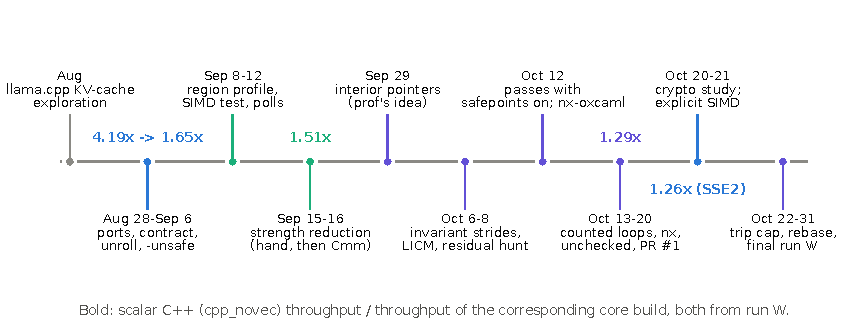
\includegraphics[width=\textwidth]{diag_timeline}
  \caption{Project timeline. Milestones show what was tried and, where a core
  build of run W corresponds, its gap to scalar C++.}
  \label{fig:timeline}
\end{figure}
